\subsection{PlayerList}

vores PlayerList klassse indeholder et array af spillere og deres accounts hver især. Derudover kender den til hvilken spiller, der har turen med currentPlayer og har et ID til hver spiller, f.eks. 1,2,3 for tre spillere.
\begin{figure}[H]
    \centering
    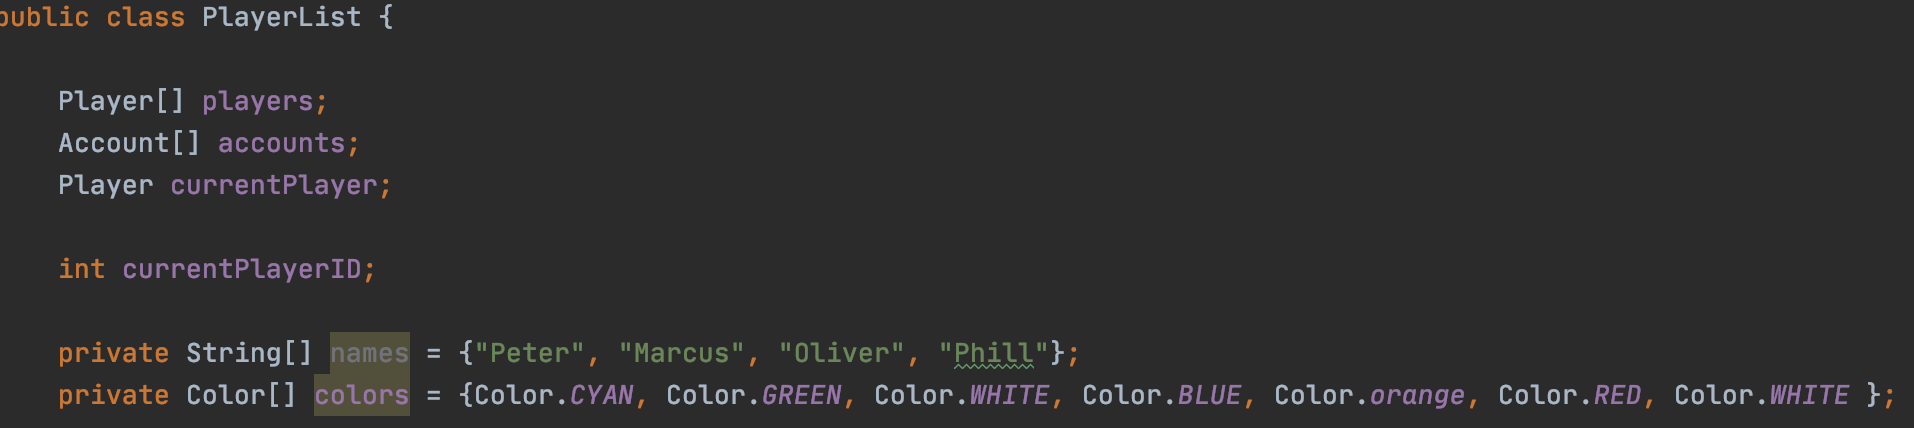
\includegraphics[width=0.7\textwidth]{sources/7_implementering/PlayerListClass.png}
    \caption{De definerede variable i PlayerList klassen}
    \label{fig:playerListklasse}
\end{figure}



\begin{figure}[H]
    \centering
    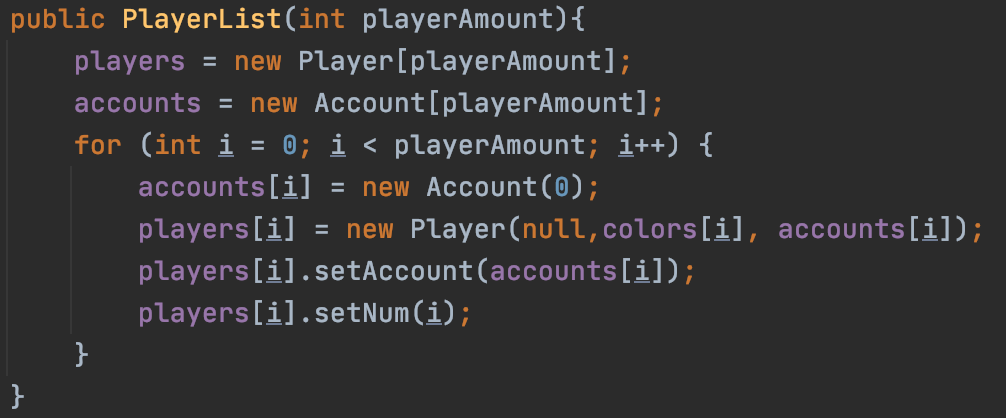
\includegraphics[width=0.7\textwidth]{sources/7_implementering/PlayerListList.png}
    \caption{PlayerList metode til spilleroprettelse}
    \label{fig:playerListmetode}
\end{figure}
PlayerList klassen laver en liste med alle spillere i spillet.  Den opretter de forskellige spillere, deres accounts og giver dem et nummer hver.


\begin{figure}[H]
    \centering
    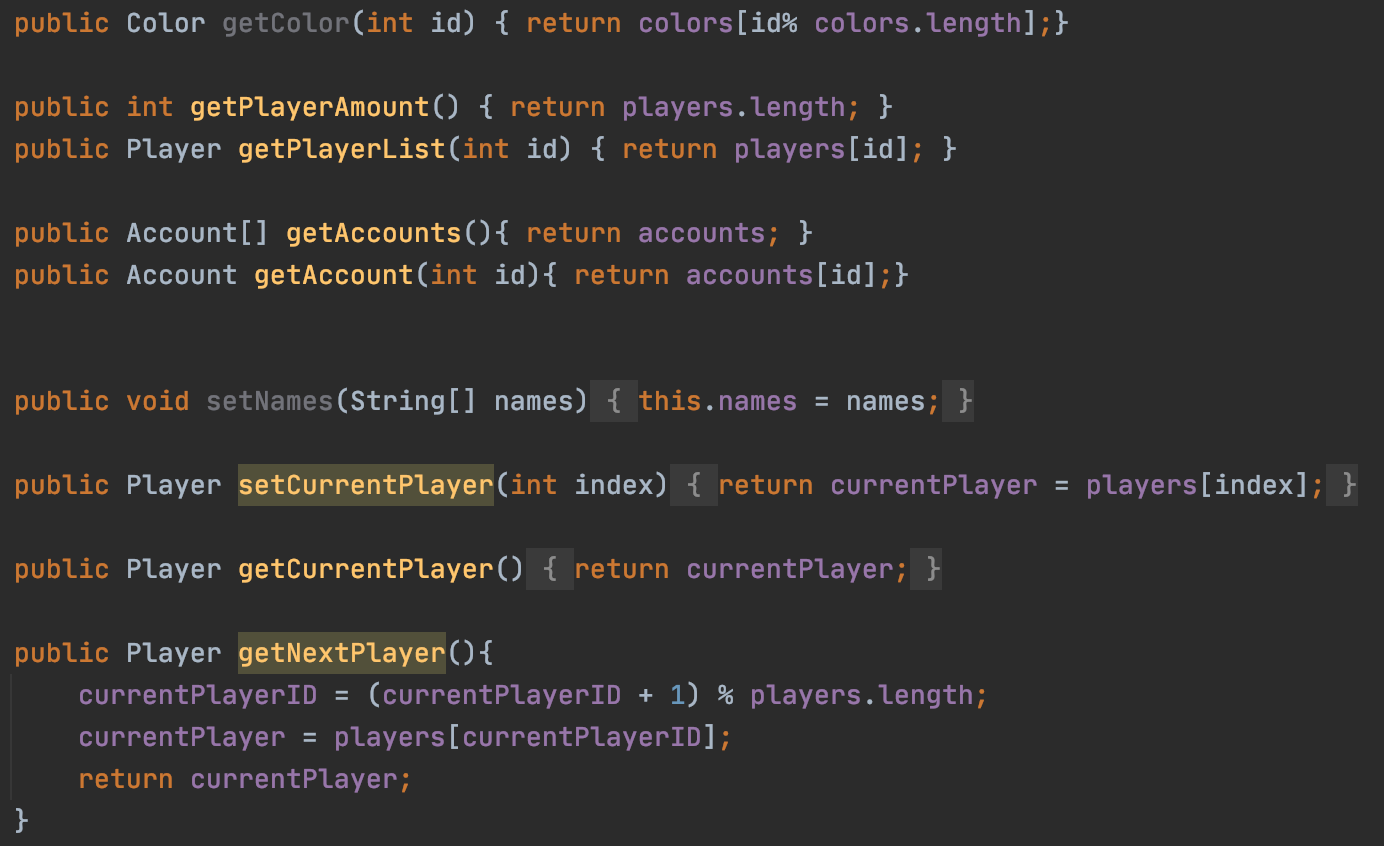
\includegraphics[width=0.7\textwidth]{sources/7_implementering/PlayerListGetSet.png}
    \caption{PlayerList Get/Set}
    \label{fig:plistGetSet}
\end{figure}
Til slut er der en række getters og setters for PlayerAmount, Accounts, CuttentPlayer og Next player. Disse holder øje med hvilken spiller. der har turen og man kan dermed få fat på hvilken spiller, der har turen og hvordan deres konto ser ud.
